%%%%%%%%%%%%%%%%%%%%%%%%%%%%%%%%%%%%%%%%%
% NIWeek 2014 Poster by T. Reveyrand
% www.microwave.fr
% http://www.microwave.fr/LaTeX.html
% ---------------------------------------
%
% Original template created by:
% Brian Amberg (baposter@brian-amberg.de)
%
% This template has been downloaded from:
% http://www.LaTeXTemplates.com
%
% License:
% CC BY-NC-SA 3.0 (http://creativecommons.org/licenses/by-nc-sa/3.0/)
%
%%%%%%%%%%%%%%%%%%%%%%%%%%%%%%%%%%%%%%%%%

%----------------------------------------------------------------------------------------
%   PACKAGES AND OTHER DOCUMENT CONFIGURATIONS
%----------------------------------------------------------------------------------------

\documentclass[a0paper,portrait]{baposter}

\usepackage[font=small,labelfont=bf]{caption} % Required for specifying captions to tables and figures
\usepackage{booktabs} % Horizontal rules in tables
\usepackage{relsize} % Used for making text smaller in some places

\usepackage{amsmath,amsfonts,amssymb,amsthm} % Math packages
\usepackage{eqparbox}

\usepackage{textcomp}

\usepackage{caption}
\usepackage{subcaption}
\usepackage{graphicx}
\usepackage{listings}
\usepackage{mathtools}
%\usepackage{verbatimbox}
%\usepackage{hyperref}

%\usepackage{pgf}

\usepackage[utf8]{inputenc}
\usetikzlibrary{shapes,arrows}
\usepackage{tikz}
\usetikzlibrary{automata,positioning}

\usepackage{multicol}

\usepackage[font=small,labelfont=bf]{caption}

\graphicspath{{figures/}} % Directory in which figures are stored

 \definecolor{bordercol}{RGB}{40,40,40} % Border color of content boxes
 \definecolor{headercol1}{RGB}{210,235,250} % Background color for the header in the content boxes (left side)
 \definecolor{headercol2}{RGB}{210,235,250} % Background color for the header in the content boxes (right side)
 \definecolor{headerfontcol}{RGB}{0,0,0} % Text color for the header text in the content boxes
 \definecolor{boxcolor}{RGB}{240,255,255} % Background color for the content in the content boxes

\tikzset{
    state/.style={
           ellipse,
           draw=black, thin,
           minimum height=0.5cm,
           minimum width=0.6cm,
           text centered,
           font=\scriptsize
           },
    horiz/.style={
           % font=\tiny,
		   inner sep=3pt,
		   font=\bf

           } ,
    point/.style={
           circle,
           minimum width = 5pt,
           fill
           }
}

\begin{document}

\setlength{\fboxsep}{0pt}

\background{ % Set the background to an image (background.pdf)
\begin{tikzpicture}[remember picture,overlay]
\draw (current page.north west)+(-2em,2em) node[anchor=north west]
{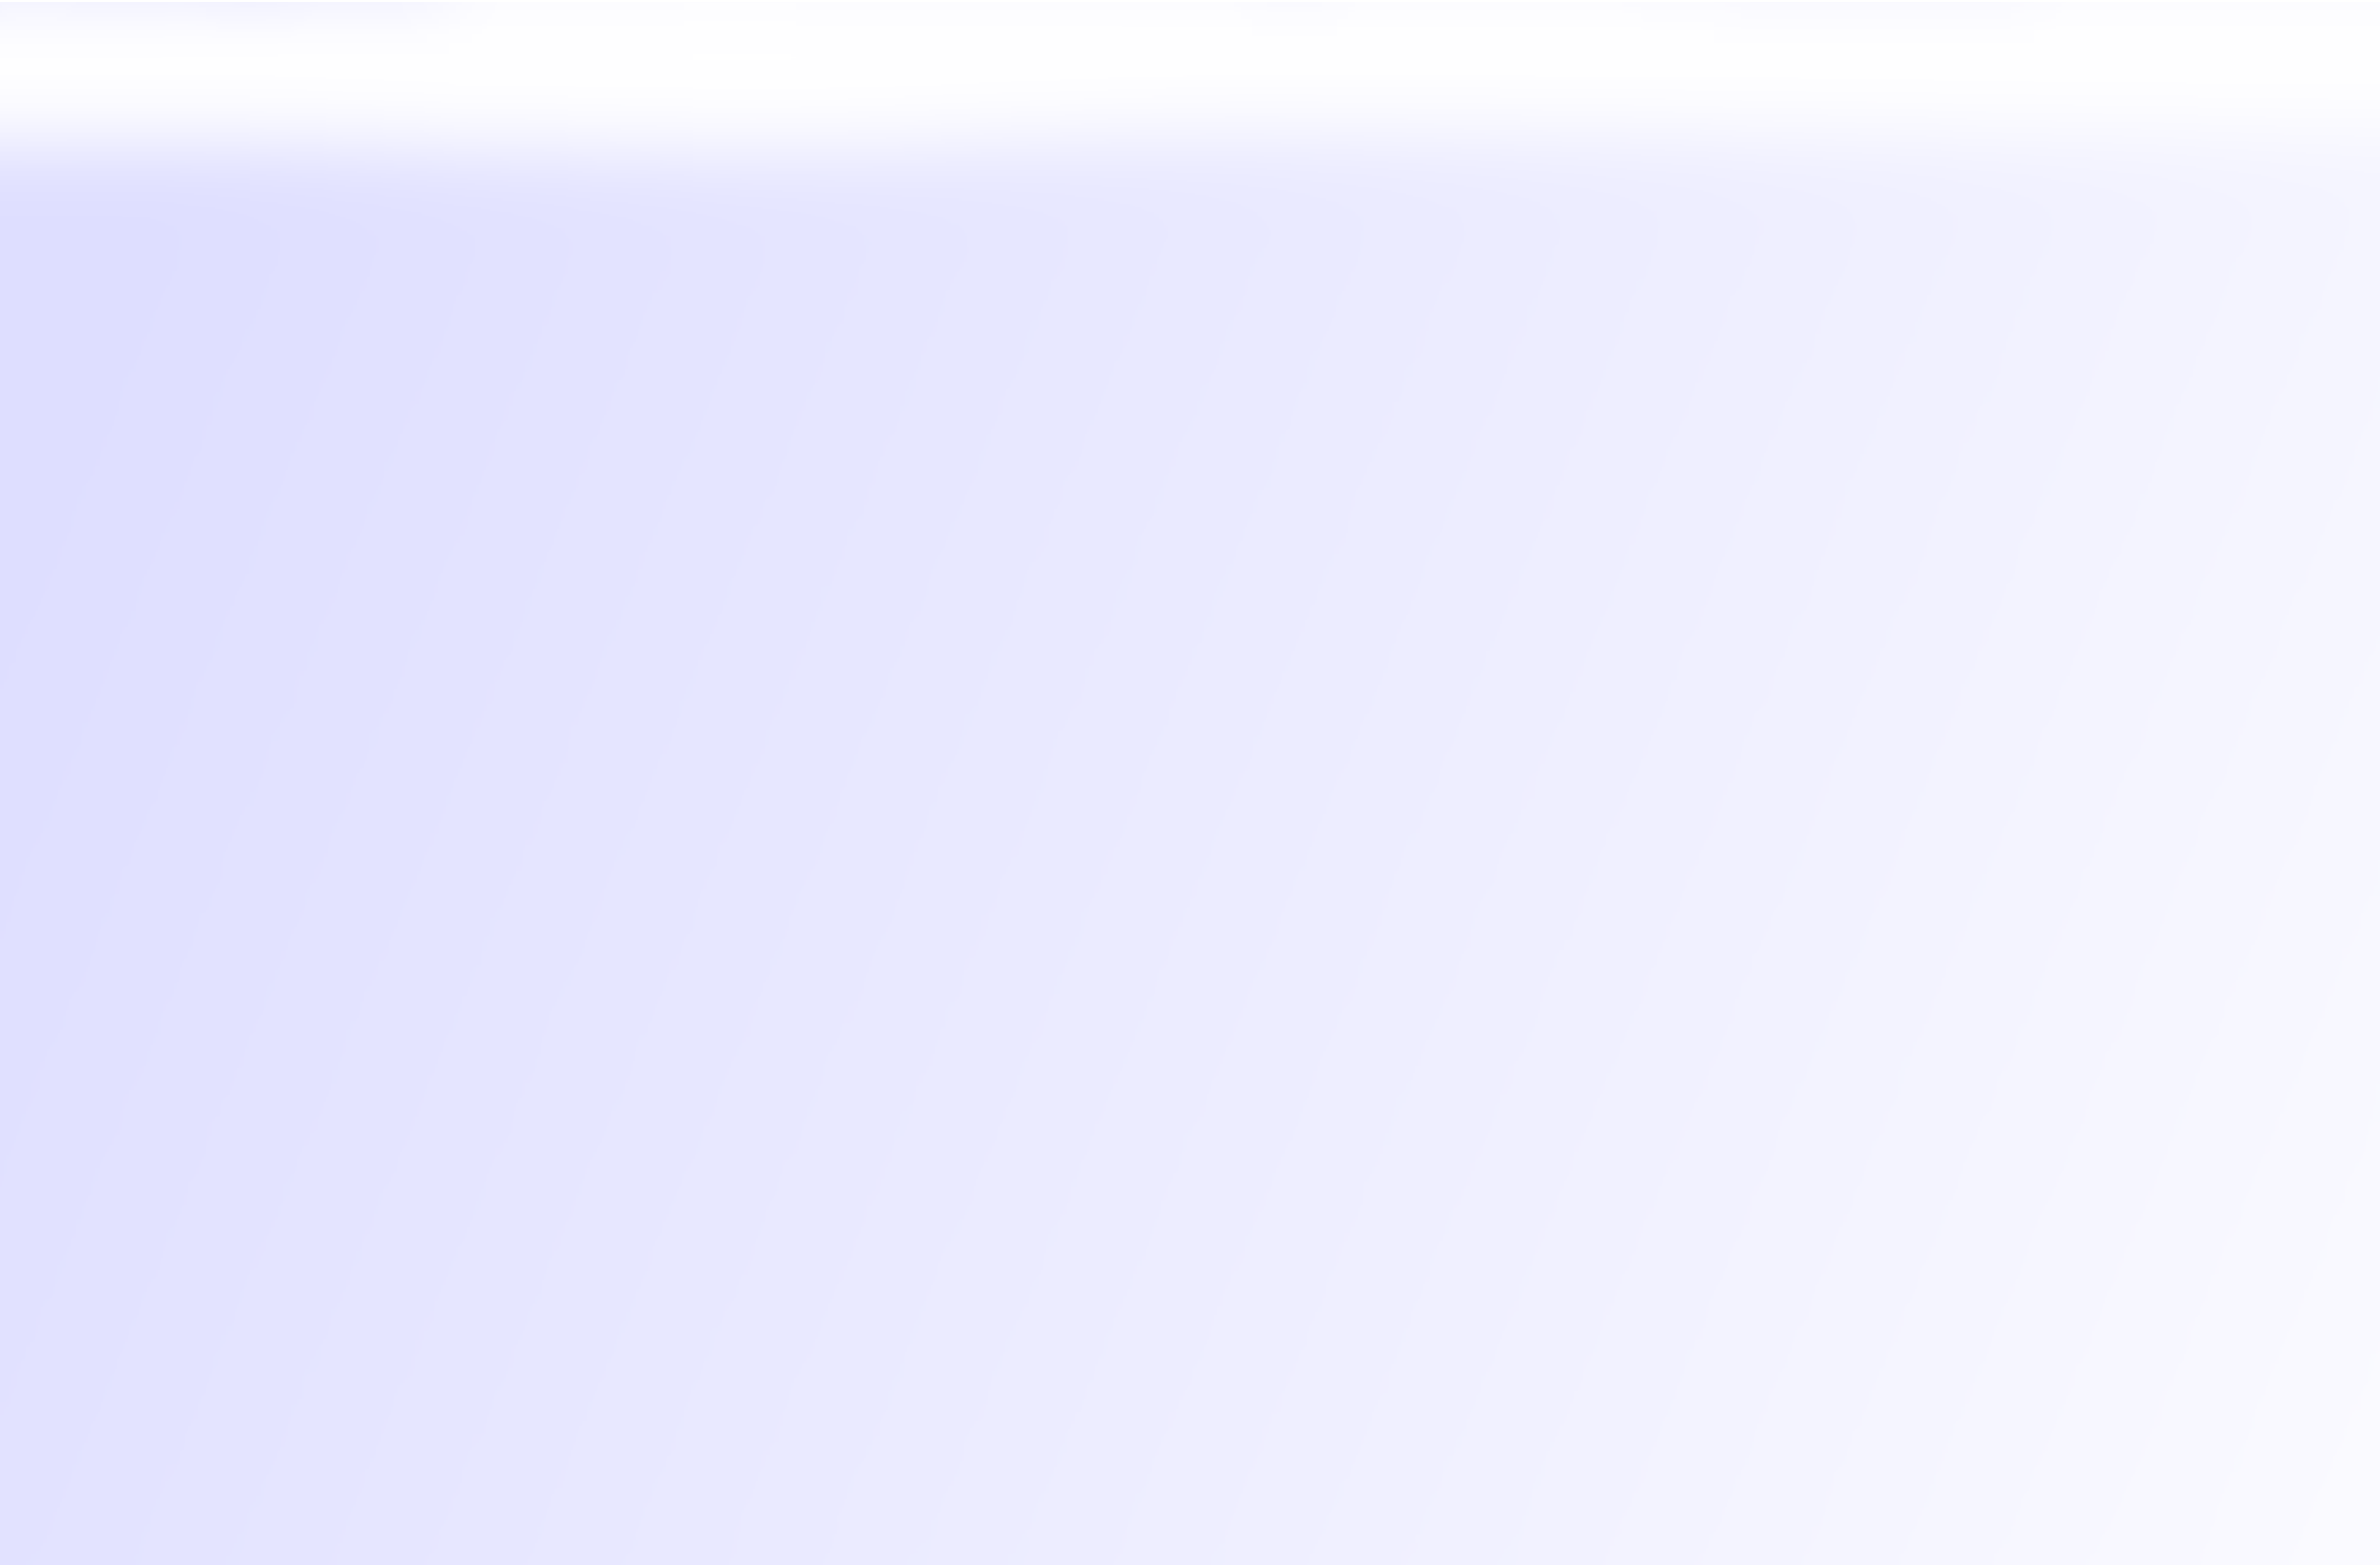
\includegraphics[height=1.1\textheight]{background}};
\end{tikzpicture}
}

\begin{poster}{
grid=false,
columns=12, % because reasons
borderColor=bordercol, % Border color of content boxes
headerColorOne=headercol1, % Background color for the header in the content boxes (left side)
headerColorTwo=headercol2, % Background color for the header in the content boxes (right side)
headerFontColor=headerfontcol, % Text color for the header text in the content boxes
boxColorOne=boxcolor, % Background color for the content in the content boxes
headershape=rectangle, % Specify the rounded corner in the content box headers
headerfont=\Large\sf\bf, % Font modifiers for the text in the content box headers
textborder=none,
background=none,
headerborder=none, % Change to closed for a line under the content box headers
boxshade=plain
}
{
\includegraphics[width=3cm]{jetbrains.png}}
%
%----------------------------------------------------------------------------------------
%   TITLE AND AUTHOR NAME
%----------------------------------------------------------------------------------------
%
{\bf \huge{Evaluation of the Context-Free Path Querying Algorithm Based on Matrix Multiplication} }
%\\  \Large \it Context-free grammars and neural networks for secondary structure} % Poster title
{\vspace{0.6em} \smaller \textbf{Semyon Grigorev} \\  % Author names
\smaller \it {JetBrains Research, Saint Petersburg State University, Russia } \\ % Author email addresses
\smaller  {kajigor@gmail.com}}
{
\includegraphics[width=2.5cm]{SPbGU_Logo.png}} % University/lab logo


%----------------------------------------------------------------------------------------
%   INTRODUCTION
%----------------------------------------------------------------------------------------
\begin{posterbox}[name=CFPQ,column=0,row=0, span=4]{Contex-Free Path Querying}

  \begin{center}
  	\textbf{The input edge-labeled directed graph}
  	
\includegraphics[width=7cm]{example_graph_transparent.png}

  	\textbf{The grammar for the language $L=\{a^n b^n\}$}\\
  	$\begin{array}{cclccl}
  	S & \rightarrow & A \ B \ | \ A \ S_1 & A & \rightarrow & \text{\emph{a}} \\
  	S_1 & \rightarrow & S \ B & B & \rightarrow & \text{\emph{b}} \\


  	\end{array}$
  \end{center}

  The result: set of node pairs such that there exists a path between them which forms a word from the $L$.

\end{posterbox}

\headerbox {Matrix Multiplication}
{name=matrices,column=0,span=4, row=2, below=CFPQ}%,bottomaligned=sol2}
{

\begin{center}
%Transitive closure of a special matrix

%\medskip

$T$ --- adjacency matrix

The grammar in the normal form

\begin{align*}
T_{ij} &=\{ N \mid N \xRightarrow[]{*} \omega,  \omega \text{ path bw } i \text{ and } j \} \\
T_{ik} \times T_{kj} &= \{ A \mid B \in T_{ik}, C \in T_{kj}, A \rightarrow B C \} \\
T^{(i)} &= T^{(i-1)} \cup (T^{(i-1)} \times T^{(i-1)})
\end{align*}

%\medskip

%\begin{minipage}[m]{\linewidth}
%\[
%\begin{pmatrix}
%	\{S\}     & \{A\}       & \varnothing & \{B, S\}    \\
%	\{S\}       & \varnothing & \{A\}       & \{S\}     \\
%	\{A, S\}  & \varnothing & \varnothing & \{S\} \\
%	\{B\}       & \varnothing & \varnothing & \varnothing \\
%\end{pmatrix}
%\]
%\end{minipage}
%
%\bigskip

Easy to run in parallel environments:

GPUs, multithreaded CPUs, clusters

\medskip

Any matrix multiplication library can be used
\end{center}
}

\headerbox {Questions}{name=questions,column=4,row=0, span=4}{%, bottomaligned=appSA}{
\begin{itemize}
  \item Does GPGPUs utilization for CFPQ improve performance in comparison with the CPU version?
  \item Is it possible to achieve higher performance by using existing libraries for operations over matrices or do we need to create our own specialized solution?
  \item Can we achieve high performance with high-level languages?
  \item Can we improve performance with sparse matrix representation?
\end{itemize}
}

\headerbox {Answers}{name=answers,column=8,row=0, span=4}{%, bottomaligned=appSA}{

\begin{itemize}
  \item GPGPUs utilization significantly increases the performance of CFPQ
  \item High performance libraries utilization is a good idea
%  \begin{itemize}
%    \item But not always: M4RI (CPU) is better then cuSPARSE (GPGPU)
%  \end{itemize}
  \item Automatic translation from a high-level language to GPGPU language provides a good balance between performance and implementation complexity
  \item Sparse matrix representation is important for performance %([Scipy] for [Sparse])
\end{itemize}

}


\headerbox {Implementations}
{name=matrices,column=4,span=4, row=2, below=questions}%,bottomaligned=sol2}
{
\begin{minipage}[t]{0.2cm}
\hspace{0.2cm}
\end{minipage}
~
\begin{minipage}[t]{0.85\textwidth}
\begin{itemize}
\item[\textbf{[Scipy]}] Sparse matrices multiplication by using \textbf{Scipy} in \textbf{Python}
\item[\textbf{[M4RI]}] Dense matrices multiplication by using \textbf{m4ri} library which implements the Method of Four Russians in \textbf{C}
\end{itemize}
\end{minipage}
}




\headerbox{We need more data!}{name=rdfs,span=12,column=0,row=2,below=matrices}{
%\begin{table}[h]
%\rowcolors{1}{}{red}
\begin{minipage}[t]{0.5\textwidth}
\begin{tabular}{| p{1.5cm} | c | c | c | c | c | c | c |}
    \hline
    \multicolumn{3}{|c|}{RDF}        & \multicolumn{5}{|c|}{Query $G_4$}  \\
    \hline
    Name                               & \#V & \#E  & Scipy & M4RI & GPU\_N & CuSprs & CYK \\ %~\footnote{Results from X. Zhang et al, 2016, ``Context-Free Path Queries on RDF Graphs''} \\
    \hline
    \hline
    {atm-prim}                    & 291 & 685  & 3     &  2    & 1      & 269  & 515285  \\
    {biomed}                      & 341 & 711  & 3     &  5    & 1      & 283  & 420604  \\
    {pizza}                       & 671 & 2604 & 6     &  8    & 1      & 292  & 3233587 \\
    {wine}                        & 733 & 2450 & 7     &  6    & 1      & 294  & 4075319 \\
    \hline
  \end{tabular}
  \captionof{table}{Query $s \to SCOR \ s \ SCO \ | \ TR \ s \ T \ | \ SCOR \ SCO \ | \ TR \ T$}

\end{minipage}
}

\headerbox{Scaling}{name=scaling,span=12,column=0,row=2,below=rdfs}{

  \begin{tabular}{| l | c | c | c | c | }
      \hline
      Graph              & Scipy   & M4RI      & GPU\_N & CuSprs  \\
      \hline
      \hline
      \small{G10k-0.001} & 37.286  & 2.395    & 0.215  & 35.937  \\
      \small{G10k-0.1}   & 601.182 & 1.050    & 0.114  & 395.393 \\
      \small{G40k-0.001} & -       & 97.841   & 8.393  & -       \\
      \small{G80k-0.001} & -       & 1142.959 & 65.886 & -       \\
      \hline
      \hline
      25000                & -       & 33.236   & 5.314   & -           \\
      50000                & -       & 360.035  & 44.611  & -           \\
      80000                & -       & 1292.817 & 190.343 & -           \\
      \hline
    \end{tabular}
}



\headerbox {\smaller{Contact us}}{name=contact,column=0,span=4,below=scaling}{
\scriptsize
Everything is available on GitHub:

\footnotesize{https://github.com/YaccConstructor}
}

\headerbox {\smaller{Acknowledgments}}{name=ack,column=0,span=4,below=contact}{
\scriptsize
The research is supported by the JetBrains Research grant and the~Russian Science Foundation grant 18-11-00100.
}

\headerbox{\smaller{References}}{name=references,column=4,span=8,below=scaling, bottomaligned=ack}{

	\scriptsize % Reduce the font size in this block
	\renewcommand{\section}[2]{\vskip 0.05em} % Get rid of the default "References" section title
	\nocite{*} % Insert publications even if they are not cited in the poster
	\bibliographystyle{unsrt}
	\bibliographystyle{IEEEtran}
	\bibliography{biblio} % Use biblio.bib as the bibliography file
}
\end{poster}


\end{document}
